\chapter{Datasets}

This chapter presents an overview of the datasets suitable for human pose estimation in depth images. The datasets are evaluated according to closeness to real-world conditions, the amount of data, and the accuracy of the recorded poses.


\section{The Panoptic Studio Dataset}

The dataset used in this work was created from source material provided by the Panoptic Studio \cite{Joo_2015_ICCV, Joo_2017_TPAMI}. Calibration files, predicted ground-truth skeletons, and depth images were downloaded using a modified version of the download script provided by the dataset. The GNU parallel program~\cite{Tange2011a} was used to download it at a faster rate. Some problems were experienced, as the Panoptic Studio server was quite unreliable, which resulted in significant delays, as well as corrupted files and, in return, a smaller dataset than desired.

The ground truth positions for the skeletons in the dataset were obtained using 2D human pose estimation on the HD, VGA, and Kinect cameras in the Panoptic Studio, and triangulating the matcing joints.

A set of five complete sequences were set aside as the test set to ensure that the network would not recognize any similar frames or body positions from previous sets. The dataset contains samples from a wide variety of activities, view-angles, the number of people in the scene, and body compositions.

The sequences in the dataset were recorded at approximately 30 fps. All frames and world coordinate positions at an approximate single timestep are hereby referred to as a \emph{frame}. To allow for poses to change, two samples were extracted per second. Each sequence was recorded by ten different Kinects from a height of 1 and 2 meters above the ground. This results in a total number of 10x the amount of samples listed in Table~\ref{tab:sequences}.

\begin{figure}
  \centering
  \begin{subfigure}{.6\textwidth}
    \centering
    \includegraphics[width=\linewidth]{img/depth_image}
    \caption{Depth image from \texttt{KINECTNODE6}.}
    \label{fig:depth_image}
  \end{subfigure}% 
  \begin{subfigure}{.4\textwidth}
    \centering
    \includegraphics[width=\linewidth]{img/dataset_skeletons}
    \caption{Skeletons defined in the world coordinate system.}
    \label{fig:dataset_skeletons}
  \end{subfigure}%
  \newline
  \begin{subfigure}{.5\textwidth}
    \centering
    \includegraphics[width=\linewidth]{img/shifted_reprojection_fixed}
    \caption{Skeletons reprojected to the depth image}
    \label{fig:reprojected_skeletons}
  \end{subfigure}%
  \hspace{1em}
  \begin{subfigure}{.4\textwidth}
    \centering
    \includegraphics[width=\linewidth]{img/pointcloud}
    \caption{The depth image projected to a point cloud.}
    \label{fig:point_cloud}
  \end{subfigure}%
  \caption{Combination of datapoints for sequence 160226\_haggling1, frame 144 in the Panoptic Studio Dataset~\cite{Joo_2015_ICCV}.}
  \label{fig:skeleton_depth_duo}
\end{figure}

\begin{table}
  \centering
  \begin{tabular}[h]{|c|l l c|}
    \hline
    & Category & Sequence Name & Duration (MM:SS) \\ \hline
    \multirow{17}{*}{\rotatebox[origin=c]{90}{Training / Validation}}
    & Range of Motion & 171204\_pose1 & 17:30 \\
    & Range of Motion & 171204\_pose2 & 22:30 \\
    & Range of Motion & 171204\_pose3 & 5:00 \\
    & Range of Motion & 171204\_pose5 & 15:00 \\ 
    & Range of Motion & 171204\_pose6 & 12:50 \\
    & Range of Motion & 171026\_pose1 & 13:20 \\
    & Range of Motion & 171026\_pose3 & 4:20 \\
    & Social Games & 160226\_haggling1 & 8:00 \\
    & Social Games & 160422\_haggling1 & 8:00 \\
    & Social Games & 160422\_ultimatum1 & 15:00 \\ 
    & Musical Instruments & 160906\_band1 & 1:00 \\ 
    & Musical Instruments & 160906\_band2 & 5:00 \\ 
    & Musical Instruments & 160906\_band3 & 5:00 \\ 
    & Toddler & 160906\_ian2 & 5:00 \\ 
    & Others & 170915\_office1 & 3:00 \\ 
    & Others & 160906\_pizza1 & 5:00 \\ 
    & Dance & 170307\_dance5 & 6:40 \\ \hline
    \multirow{5}{*}{\rotatebox[origin=c]{90}{Test}}
    & Range of Motion & 171204\_pose4 & 17:30 \\ 
    & Range of Motion & 171026\_pose2 & 9:00 \\ 
    & Social Games & 160224\_haggling1 & 5:00 \\ 
    & Toddler & 160906\_ian1 & 2:00 \\ 
    & Others & 170407\_office2 & 3:00 \\ \hline
  \end{tabular}
  \caption{Sequences used for training, validation and testing}
  \label{tab:sequences}
\end{table}


\section{Dataset Augmentations}

The coco19 points from the pose directories were reprojected into the depth image using the perspective camera model

\begin{equation}
  \textbf{\emph{u}} = K\begin{bmatrix}1 & 0 & 0 & 0 \\ 0 & 1 & 0 & 0 \\ 0 & 0 & 1 & 0\end{bmatrix}
  \begin{bmatrix}R_{3 \times 3} & \textbf{\emph{t}}_{3 \times 1} \\ \textbf{0}_{1 \times 3} & 1\end{bmatrix}\textbf{\emph{\~{X}}}
\end{equation}

The matrix \emph{K} is the camera intrinsics and describes how to transform the point from the normalized image-plane to the pixel coordinates in the image.
\begin{equation}
  K = \begin{bmatrix}f_{u} & s & c_{u} \\ 0 & f_{v} & c_{v} \\ 0 & 0 & 1\end{bmatrix}
\end{equation}
where $f_{u}, f_{v}$ is the focal lengths in column/row direction, \emph{s} is the skew and $c_{u}, c_{v}$ is the center of the image in column/row direction.

In the dataset, each sequence provided a file containing the \emph{K} matrices for all the sensors in an unordered list. It was therefore assumed that the placement in the list corresponded to the number of the sensor. However, the extrinsic parts of these did not yield correct results. Another set of extrinsic rotation/translation matrices were provided in a different file where the sensor number \emph{was} identified. Still, these extrinsic parameters were calibrated for the color camera of each sensor. Since the depth camera and color camera of the Kinect are placed approximately 20cm from each other, a vector $\Bigl[\begin{smallmatrix}0.02\\0\\0\end{smallmatrix}\Bigr]$ was added after calculating the extrinsic part of the model to compensate. The resulting projections can be seen in figure~\ref{fig:reprojected_skeletons}. Still, the \emph{K} matrices had to be sourced from the unordered list and introduced uncertainty about whether the datasets will be accurate. Since the Kinect cameras are the same model, and after all very similar, this uncertainty were chosen to be ignored.

\begin{figure}
  \begin{subfigure}{.5\textwidth}
    \centering
    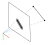
\includegraphics[width=\linewidth]{img/projection}
    \caption[Projection]{A limb is projected onto the image plane}
    \label{fig:projection}
  \end{subfigure}
  \begin{subfigure}{.5\textwidth}
    \centering
    \includegraphics[width=\linewidth]{img/closest_points}
    \caption[Beam]{The beam cast through a pixel in the image plane}
    \label{fig:projection}
  \end{subfigure}
  \caption{}
  
\end{figure}

\begin{equation}
  \label{eq:epanechnikov}
  K(x, y) =
  \begin{cases}
    \frac{2}{\pi\sigma^{2}}(1 - ((\frac{x}{\sigma})^{2} + (\frac{y}{\sigma})^{2})) & \text{if } |(\frac{x}{\sigma})^{2} + (\frac{y}{\sigma})^{2}| \leq 1\\
    0 & \text{otherwise}
  \end{cases}
\end{equation}

\begin{figure}
  \begin{subfigure}{.4\textwidth}
    \centering
    \includegraphics[width=\linewidth]{img/epanechnikov_2d}
    \caption{A 2D Epanechnikov \cite{epanechnikov_1969} kernel.}
    \label{fig:epanechnikov}
  \end{subfigure}%
  \begin{subfigure}{.6\textwidth}
    \centering
    \includegraphics[width=\linewidth]{img/target_maps}
    \caption{Variable kernel width}
    \label{fig:magnitude}
  \end{subfigure}
  \caption{Kernel variation based on distance}
  \label{fig:kernelvariation}
\end{figure}

Target limb-maps for each frame were created by projecting all instances of a certain type of limb onto an empty matrix of the same dimensions as the depth frame, illustrated in Figure~\ref{fig:projection}. Because of the discrete nature of a depth image, projecting the 3D limb into the image will yield a set of pixels. For each pixel point along the line created by the projected limb, the depth was calculated by finding the closest points of the infinite 3D line created by the limb and the projected beam from the camera coordinate system through the 3D point formed by the pixel. The closest points of the resulting skewed 3D lines was calculated by solving the linear equation set~\ref{eq:closestpoints}, and plugging the results in to the corresponding line-equations.

A 2D Epanechnikov Kernel with a $\sigma$ varying based on the distance were then used to calculate the magnitude for each of the 3D vectors pointing in the direction of the limb in question. The distance used to calculate the width of the kernel were stored for later comparison. Where limbs would occlude each other, the values for the pixel with the closest point were retained. The reason for varying the $\sigma$ was to simulate that the shell of points around a limb would appear smaller at a greater distance. Because a normal epanechnikov kernel would change the max value of the center of the line, the equation was simplified to a quadratic function~\ref{eq:simplequad}.

\begin{equation}
  \label{eq:simplequad}
  K(x, y) =
  \begin{cases}
    1 - ((\frac{x}{\sigma(x, y)})^{2} + (\frac{y}{\sigma(x, y)})^{2}) & \text{if } |(\frac{x}{\sigma(x, y)})^{2} + (\frac{y}{\sigma(x, y)})^{2}| \leq 1\\
    0 & \text{otherwise}
  \end{cases}
\end{equation}

\begin{equation}
  \label{eq:depth}
  d =
  \begin{cases}
    \max(\|\mathbf{j_1}\|, \|\mathbf{j_2}\|) & \text{if} \|\mathbf{v}\| >  \max(\|\mathbf{j_1}\|, \|\mathbf{j_2}\|) \\
    \min(\|\mathbf{j_1}\|, \|\mathbf{j_2}\|) & \text{if} \|\mathbf{v}\| <  \min(\|\mathbf{j_1}\|, \|\mathbf{j_2}\|) \\    
    \|\mathbf{v}\| & \text{otherwise}
  \end{cases}
\end{equation}

\begin{equation}
  \label{eq:closestpoints}
  \begin{split}
  L_1 = (l_{1x}, l_{1y}, l_{1z}), \; u_1 = (u_{1x}, u_{1y}, u_{1z}) \\
  L_2 = (l_{2x}, l_{2y}, l_{2z}), \; u_1 = (u_{2x}, u_{2y}, u_{2z}) \\[20pt]
  \begin{bmatrix}
    u_{1x}^{2} + u_{1y}^{2} + u_{1z}^{2} & -(u_{1x} * u_{2x} + u_{1y} * u_{2y} + u_{1z} * u_{2z}) \\
    u_{1x} * u_{2x} + u_{1y} * u_{2y} + u_{1z} * u_{2z} & -(u_{2x}^{2} + u_{2y}^{2} + u_{2z}^{2})
  \end{bmatrix} \\
  = 
  \begin{bmatrix}
    u_{1x} (l_{2x} - l_{1x}) + u_{1y} (l_{2y} - l_{1y}) + u_{1z} (l_{2z} - l_{1z}) \\
    u_{2x} (l_{2x} - l_{1x}) + u_{2y} (l_{2y} - l_{1y}) + u_{2z} (l_{2z} - l_{1z})
  \end{bmatrix}
  \end{split}
\end{equation}

Equation~\ref{eq:depth} describes how $\sigma$ changes by the value in the depth image $D$. The constant $c$ is chosen by the width of the limb in pixels at a certain distance.

The resulting magnitudes for the limbs are illustrated by the declining intensity in figure~\ref{fig:magnitude}. The produced sample tensors are illustrated in figure~\ref{fig:targets}. For each sequence, a ``long'' tensor is made. The first slice of the tensor is the depth image, of size $1 \times w \times h$. Next, the limb maps are stored. They contain the decomposition of the vector, $x, y, z$ in each pixel. This part of the sample, therefore, has the size $3M \times w \times h$ for \emph{M} limbs. Last is the Joint Maps, which contain both the distance to the center of the joint and the confidence for each pixel. The confidences are also simulated by placing a kernel made by equation~\ref{eq:simplequad} at the projected location for the joint, with a $\sigma$ based on the distance from the camera to the joint. This results in the size $2N \times w \times h$ for \emph{N} joints. In addition to the target maps in figure~\ref{fig:targets}, the resulting dataset also contains a vector with the position of all joints in the image in the coordinate frame of the camera. This is to provide ground truth targets for the articulation network if the joint is occluded in the joint map.

A single tensor of samples was created for each sequence. At training time, all sequences except the test sequences were combined to a single dataset which was shuffled.

\begin{figure}
  \centering
  \includegraphics[width=.8\textwidth]{img/targets}
  \caption[Data Tensors]{The sturcture of the created dataset}
  \label{fig:targets}
\end{figure}

The raw dataset is captured at 30 fps for each of the ten kinects in the Panoptic Studio. To not capture similar poses in the dataset, three frames are sampled from each kinect per second. In addition, the order the kinects are sampled is shuffled after each sampling round.
